\chapter{TASOM}
O TASOM foi criado com o intuito de modificar o SOM para retirar a dependência temporal e adicionar mecanismos com capacidade de detectar mudança. O TASOM automaticamente ajusta seus parâmetros de aprendizagem para incorporar as mudanças do conjunto de entrada nos pesos dos neurônios. O algoritmo será resumido nas próximas sub-seções deste capítulo. Os parâmetros iniciais do sistema são:
\begin{enumerate}
\item Altura do Mapa: O número de linhas do mapa.
\item Largura do Mapa: O número de colunas do mapa.
\item Raio de Vizinhança Inicial: Tamanho do raio de vizinhança inicial.
\item Taxa de Aprendizagem Inicial: Valor da taxa de aprendizagem incial.
\item Coeficiente de Aprendizagem: Constante que altera o cálculo da taxa de aprendizagem, quanto maior ele for maior será a plasticidade da rede.
\item Coeficiente de Vizinhança: Constante que altera o cálculo do raio de vizinhança, quanto maior ele for mais lentamente será a diminuição do raio de vizinhança.
\item SG: Constante que altera o cálculo do raio de vizinhança, possui efeito similar ao coeficiente de vizinhança, mas seu efeito é menor.
\item SF: Constante que altera o cálculo da taxa de aprendizado, possui efeito similar ao coeficiente de aprendizagem, mas seu efeito é menor.
\item Alfa:Constante que atua no fator de escalabilidade, quanto maior ela for maior será a plasticidade da rede.
\item Beta:Constante que atua no fator de escalabilidade, quanto maior ela for maior será a convergência da rede.
\end{enumerate}
 

\section{Inicialização}
A primeira etapa do TASOM é a criação do mapa. A dimensionalidade do mapa pode ser de qualquer tamanho, para os estudos aqui realizados foi escolhido a criação de um mapa bi-dimensional. Para cada neurônio é necessário a criação de um conjunto de pesos, variável de aprendizado e raio de vizinhança, estes atributos são individuais de cada neurônio. A variável de aprendizado e o raio de vizinhança são parâmetros iniciais da redes e o vetor de pesos deve ser inicializado com valores randômicos e pequenos. Existem algumas restrições que devem ser observadas nos parâmetros iniciais: A taxa de aprendizado inicial de ser inicializada com um valor próximo de 1. As constantes Alfa, Beta, Coeficiente de Aprendizagem e Coeficiente de Vizinhança devem ser valores entre 0 e 1. O raio de vizinhança inicial deve ser maior do que 0. O fator de escalabilidade inicial dever ser positivo, e, preferencialmente, igual a 1. Os valores das funções internas do fator de escalabilidade, Ek e E2k, devem ser inicializados com valores randomicamente pequenos. 

\section{Regra de Micro-Coesão}
Para o cálculo do raio de vizinhança de cada neurônio o TASOM leva em consideração o quão coeso o neurônio está de seus vizinhos. Quanto maior for esta coesão, menor será a atualização no tamanho novo do raio de vizinhança. Para aferir a micro-coesão é necessário determinar qual a regra de vizinhança do mapa. Esta regra varia de acordo com a aplicação da rede e a dimensionalidade do mapa. A figura 21 mostra uma regra de vizinhança para mapas quadrados, onde: \textit{NH} é o conjunto de vizinhos do neurônio \textit{i} e \textit{M} é a dimensionalidade do mapa. 


\begin{figure}[!h]
\centering
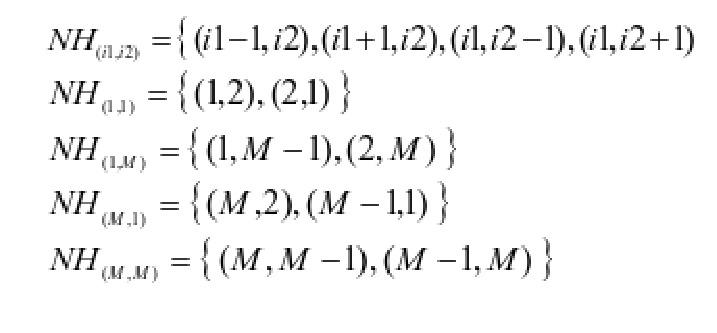
\includegraphics[keepaspectratio=true,scale=0.50]
{figuras/dimensionalidade.eps}
\caption{Regra de Vizinhança - \citeonline{tasom2001}}
\label{data_titatic}
\end{figure}

\section{Escolha do Neurônio Vencedor}
Para o cálculo do neurônio vencedor, é necessário comparar o dado de entrada com os pesos de cada um dos neurônios do mapa. Aquele neurônio que for mais parecido com a entrada será escolhido como neurônio vencedor. Para realizar esta comparação é necessário estabelecer um método de medir a distância entre a entrada e os neurônios, o neurônio mais parecido será aquele que apresentar menor distância com a entrada. A figura 22 mostra este cálculo utilizando a distância euclidiana, onde: \textit{X(n)} é o vetor de entrada e \textit{W(n)} o vetor de pesos dos neurônios. Esta etapa também é encontrada no SOM.

\begin{figure}[!h]
\centering
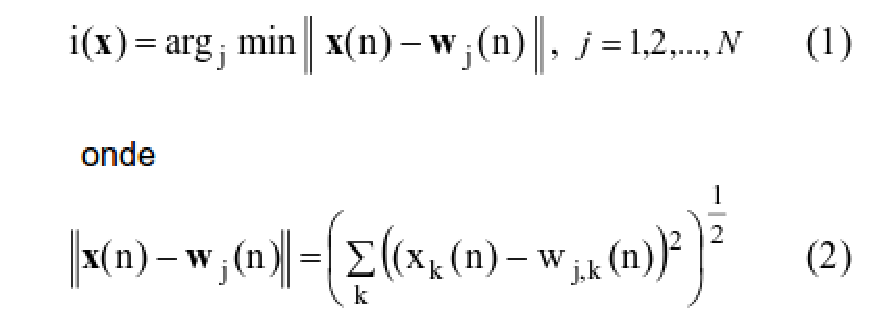
\includegraphics[keepaspectratio=true,scale=0.50]
{figuras/vencedor.eps}
\caption{Descoberta do Neurônio Vencedor - \citeonline{tasom2001}}
\label{data_titatic}
\end{figure}

\section{Atualização do Raio de Vizinhança}
Após a descoberta do neurônio vencedor, é necessário atualizar seu raio de vizinhança de acordo com a equação da figura 23, onde: $\sigma i$ é o raio de vizinhança do neurônio \textit{i}. $\beta$ é o Coeficiente de Vizinhança. \textit{g} é uma função denota por \textit{(M $\sqrt{2}$ - 1)(1 - $\frac{1}{1 + z}$)}, \textit{M} é a dimensionalidade do mapa. \textit{SG} é a constante inicialmente parametrizada. \textit{sl(n)} é o fator de escalabilidade. E, \textit{\#(NHi)} é a cardinalidade do conjunto de vizinhos. Esta cardinalidade dividida pelo somatório das distâncias entre o neurônio vencedor e seus vizinhos é a micro-coesão. 

\begin{figure}[!h]
\centering
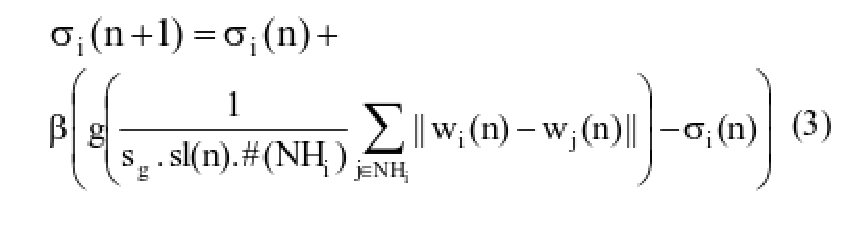
\includegraphics[keepaspectratio=true,scale=0.50]
{figuras/viz.eps}
\caption{Atualização do Raio de Vizinhança - \citeonline{tasom2001}}
\label{data_titatic}
\end{figure}

\section{Atualização da Taxa de Aprendizagem}
A taxa de aprendizagem de todos os neurônios deve ser atualizada de acordo com a equação da figura 24, onde: $\eta j$(n) é a taxa de aprendizagem do neurônio atual. \textit{$\alpha$} é o Coeficente de Aprendizagem. \textit{f} é uma função denotada por 1 - $\frac{1}{1 + z}$. \textit{SF} é a constante inicialmente parametrizada. \textit{sl(n)} é o fator de escalabilidade. E, $\Vert X(n) - Wj(n)\Vert$ é a norma da distância entre os pesos do neurônio e a entrada. 

\begin{figure}[!h]
\centering
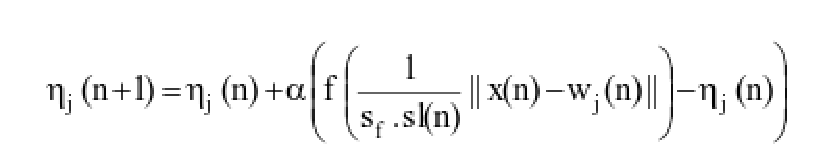
\includegraphics[keepaspectratio=true,scale=0.65]
{figuras/learn.eps}
\caption{Atualização da Taxa de Aprendizagem - \citeonline{tasom2001}}
\label{data_titatic}
\end{figure}

\section{Atualização dos Pesos}
Nesta etapa é necessário atualizar o peso de todos os neurônios seguindo a equação 25, onde: \textit{Wj(n)} é o vetor de pesos do neurônio \textit{n}. $\eta j$(n+1) é a taxa de aprendizado daquele neurônio já atualizada. \textit{$\mathbf{h}_ij(x)$(n+1)} é a mesma equação que determina a influência da atualização de acordo com distância do neurônio vencedor do SOM, pode ser encontrada na figura 18. X(n) - $\mathbf{W}_j$ é a diferença entre a entrada e o peso do neurônio atual.

\begin{figure}[!h]
\centering
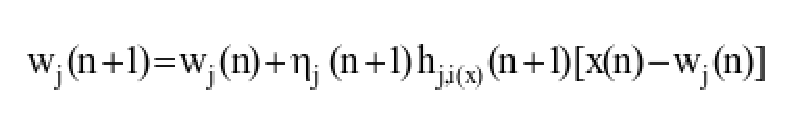
\includegraphics[keepaspectratio=true,scale=0.65]
{figuras/synp.eps}
\caption{Atualização dos Pesos - \citeonline{tasom2001}}
\label{data_titatic}
\end{figure}


\section{Fator de Escalabilidade}
A atualização do fator de escalabilidade seque a equação da figura 26, que por sua vez segue as equações das figuras 27 e 28, onde: $\mathbf \alpha _s$ é a constante Alfa parametrizada inicialmente. $\mathbf \beta _s$ é a constante Beta parametrizada inicialmente. E, $(z)^+$ = z se z > 0, ou z = 0 caso contrário.

\begin{figure}[!h]
\centering
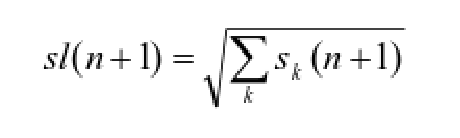
\includegraphics[keepaspectratio=true,scale=0.65]
{figuras/sl.eps}
\caption{Fator de Escalabilidade - \citeonline{tasom2001}}
\label{data_titatic}
\end{figure}

\begin{figure}[!h]
\centering
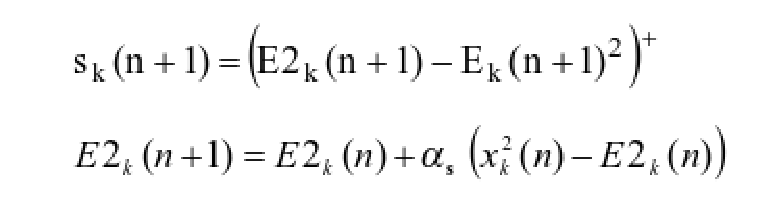
\includegraphics[keepaspectratio=true,scale=0.65]
{figuras/sk.eps}
\caption{Parcial da Equação da figura 26 - \citeonline{tasom2001}}
\label{data_titatic}
\end{figure}

\begin{figure}[!h]
\centering
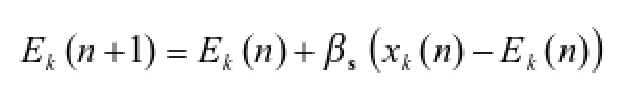
\includegraphics[keepaspectratio=true,scale=0.65]
{figuras/ek.eps}
\caption{Parcial da Equação da figura 26 - \citeonline{tasom2001}}
\label{data_titatic}
\end{figure}

























